\textbf{\LARGE osn 2. Производная и дифференциал функций одной и нескольких переменных. Достаточные условия дифференцируемости.}

\textbf{Производной функции} $f(x)$ в точке $x_0$ называется предел при $\Delta x \to 0$ разностного отношения (если этот предел существует): $f'(x_0) = \lim \limits_{\Delta x \to 0}\frac{\Delta y}{\Delta x} = \lim \limits_{\Delta x \to 0} \frac{f(x_0+\Delta x)-f(x_0)}{\Delta x}$ ($x_0 + \Delta x \in$ области определения функции)

\bigbreak
Функция $f(x)$ называется \textbf{дифференцируемой в точке} $x_0$, если она определена в некоторой окрестности этой точки, а приращение $\Delta y$ этой функции в точке $x_0$, отвечающее приращению аргумента $\Delta x$, может быть представлено в виде $\Delta y = A \Delta x+ \omega(\Delta x)$, где $A$ --- не зависящее от $\Delta x$ конечное число, а $\omega(\Delta x) = o(\Delta x)$ при $\Delta x \to 0$

\bigbreak
Функция $u = f(x_1,\dots,x_m)$ называется \textbf{дифференцируемой в точке $M(x_1,\dots,x_m)$}, если её полное приращение в точке $M$ можно представить: 
$$ \Delta u= A_1 \Delta x_1 +\dots+A_m \Delta x_m + \alpha_1 \Delta x_1 +\dots+ \alpha_m \Delta x_m $$
где $A_1, \dots, A_m$ --- некоторые не зависящие от $\Delta x_1, \dots, \Delta x_m$ числа, а $ \alpha_1, \dots, \alpha_m$ --- бесконечно малые при $\Delta x_1 \to 0, \dots, \Delta x_m \to 0$ функции, равные 0 при $\Delta x_1 = \dots = \Delta x_m = 0$

\bigbreak
\textbf{Частная производная функции} $f(x_1,\dots,x_m)$ по переменной $x_i$ --- это предел отношения приращения функции по $x_i$ к приращению этой переменной, при стремлении этого приращения к нулю: $$ \frac{\partial f}{\partial x_i} = \lim\limits_{\Delta x \to 0}\frac{ f(x_1,\dots,x_i +\Delta x,\dots,x_m)-f(x_1,\dots,x_i,\dots,x_m)}{\Delta x}$$

\bigbreak
\textbf{Дифференциалом} $du$ дифференцируемой в $M(x_1,\dots,x_m)$ функции $u = f(x_1,\dots,x_m)$ называется главная линейная относительно приращений аргументов часть приращения этой функции в точке $M.$
$$du=A_1\Delta x_1 +\dots+A_m \Delta x_m = \frac{\partial u}{\partial x_1}\Delta x_1 +\dots+ \frac{\partial u}{\partial x_m}\Delta x_m$$

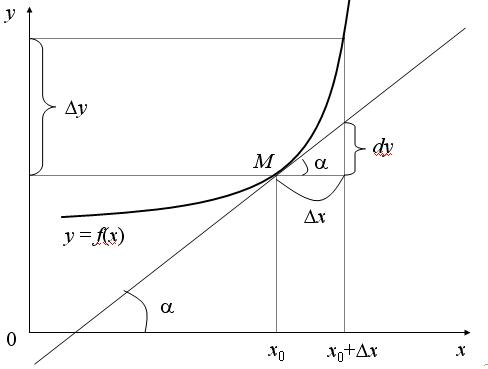
\includegraphics[scale=0.65]{pics/osn02_derivative.jpg}

\textbf{Критерий дифференцируемости для функции одной переменной}. Функция одной переменной $f(x)$ дифференцируема в точке $x_0$ $\iff$ она имеет в этой точке конечную производную.

\begin{proof} 
$(\implies) \Delta y = A \Delta x + \alpha(\Delta x)\Delta x \Rightarrow$ \{$\mathLet \Delta x \neq 0$\} $\Rightarrow \frac{\Delta y}{\Delta x}=A + \alpha(\Delta x) \Rightarrow \lim\limits_{\Delta x \to 0}\frac{\Delta y}{\Delta x}=A \Rightarrow f'(x) = A$\\
$(\impliedby) \mathLet \exists f'(x) < \infty. \mathLet \alpha(\Delta x)=\frac{\Delta y}{\Delta x}-f'(x)$, домножим на $\Delta x: \Delta y=f'(x)\Delta x+\alpha(\Delta x)\Delta x$
\end{proof}
\bigbreak

\textbf{Необходимое условие дифференцируемости для функций нескольких переменных.} Если $u = f(x_1,\dots,x_m)$ дифференцируема в $M(x_1,\dots,x_m)$, то в этой точке $\exists$ частные производные по всем аргументам, причём $\frac{\partial u}{\partial x_i} = A_i$, где $A_i$ определяются из условия дифференцируемости функции.

\begin{proof}
Из условия дифференцируемости вытекает, что частные приращения 
$\Delta u_i = A_i\Delta x_i+\alpha_i\Delta x_i$
$\Rightarrow \frac{\Delta u_i}{\Delta x_i} = A_i + \alpha_i $
$\Rightarrow \{\alpha_i \to 0$ при $\Delta x_i \to 0\} $
$\Rightarrow \lim\limits_{\Delta x_i \to 0}\frac{\Delta u_i}{\Delta x_i}=A_i$
\end{proof}

Условие не является достаточным, пример: $f(x, y) = \sqrt{\left|xy\right|}$ -- $\exists$ ч.п. 
$f'_x = \frac{1}{2} \sqrt{\frac{y}{x}}$, $f'_y = \frac{1}{2} \sqrt{\frac{x}{y}}$, но не дифф. в т. 0.
\bigbreak

\textbf{Достаточное условие дифференцируемости функций нескольких переменных.} Если $u = f(x_1,\dots,x_m)$ имеет частные производные по всем аргументам в некоторой окрестности точки $M_0(x^0_1, \dots, x^0_m)$, причём все эти частные производные непрерывны в точке $M_0$, то функция дифференцируема в точке $M_0$.

\begin{proof}
Для функции двух переменных $u=f(x,y)$: $\mathLet$ ч.п. $f'_x$ и $f'_y$ $ \exists$ в окр-ти точки $M_0(x_0,y_0)$ и непрерывны в этой точке, $\mathLet$ $M(x_0+\Delta x, y_0 + \Delta y)$ принадлежит указанной окрестности. \\
$\Delta u=f(x_0+\Delta x, y_0+\Delta y) - f(x_0, y_0) = [f(x_0+\Delta x, y_0+\Delta y)-f(x_0, y_0+\Delta y)] + [f(x_0, y_0+\Delta y) - f(x_0, y_0)]$ \\
$[f(x_0+\Delta x, y_0+\Delta y)-f(x_0, y_0+\Delta y)]$ -- приращение ф-ии одной переменной на сегменте $[x_0, x_0+\Delta x]$. Т.к. $u = f(x,y)$ имеет ч.п., то $f(x, y_0+\Delta y)$ дифф-ма и ее производная по $x = f'_x$. Применим к указанному приращению формулу Лагранжа: \\
$[f(x_0+\Delta x, y_0+\Delta y)-f(x_0, y_0+\Delta y)] = f'_x(x_0+\theta_1\Delta x, y_0+\Delta y)\Delta x, ~ \theta_1 \in (0,1)$.\\
Аналогично 
$[f(x_0, y_0+\Delta y)-f(x_0, y_0)] = f'_y(x_0, y_0+\theta_2\Delta y)\Delta y, ~ \theta_2 \in (0,1)$.

$f'_x$ и $f'_y$ непр. в т. $M_0 \Rightarrow f'_x(x_0+\theta_1\Delta x, y_0+\Delta y)=f'_x(x_0,y_0) + \alpha$, $f'_y(x_0, y_0+\theta_2\Delta y)\Delta y=f'_y(x_0,y_0) + \beta$, где $\alpha$ и $\beta$ -- беск. малые при $\Delta x \to 0, ~ \Delta y \to 0$ ф-ии. \\
Отсюда: $\Delta u=f'_x(x_0,y_0)\Delta x + f'_y(x_0,y_0)\Delta y + \alpha\Delta x + \beta\Delta y \Rightarrow u = f(x,y)$ -- дифф-ма в точке $M_0$.

Для ф-ии $m$ переменных $u=f(x_1, \dots, x_m)$ аналогично, представив $\Delta u$  в виде: \\
$\Delta u = f(x^0_1+\Delta x_1, \dots, x^0_m+\Delta x_m) - f(x^0_1, \dots, x^0_m) = \sum_{i=1}^{m}[f(x^0_1, \dots, x^0_i+\Delta x_i, \dots, x^0_m+\Delta x_m) - f(x^0_1, \dots, x^0_i, x^0_{i+1}+\Delta x_{i+1}, \dots, x^0_m+\Delta x_m)]$
\end{proof}




% -------- source --------
